
%%%%%%%%%%

%\begin{figure}[h]

\centering
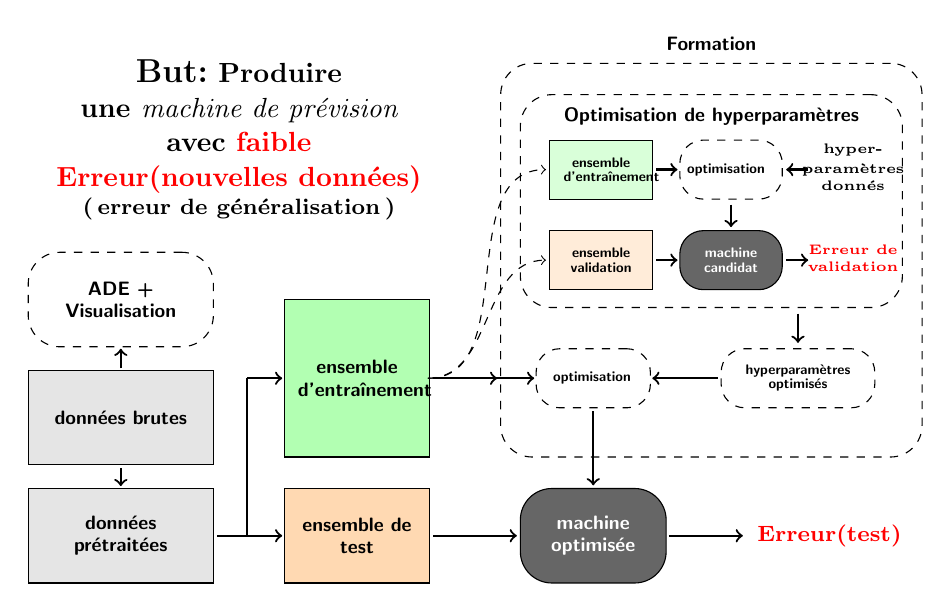
\begin{tikzpicture}
[node distance = 1cm, auto,font=\scriptsize,
% STYLES
every node/.style={node distance=3cm},
% The comment style is used to describe the characteristics of each force
comment/.style={rectangle, inner sep= 5pt, text width=4cm, node distance=0.25cm, font=\scriptsize\sffamily},
% The force style is used to draw the forces' name
force/.style={rectangle, draw, fill=black!10, inner sep=5pt, text width=2cm, text badly centered, minimum height=1.2cm, font=\bfseries\scriptsize\sffamily}] 

\pause
\node at (1.5,6.9) {\large\bf But:\;\normalsize Produire};
\node at (1.5,6.4) {\normalsize\bf une \it machine de pr\'{e}vision};
\node at (1.5,6.0) {\normalsize\bf avec {\color{red}faible}};
\node at (1.5,5.525) {\normalsize\bf\color{red}Erreur(nouvelles donn\'{e}es)};
\node at (1.5,5.15) {\footnotesize\bf(\,erreur de g\'en\'eralisation\,)};

%%%  ~~~~~~~~~~  %%%

\pause
\node [force] at (0,2.5) {donn\'{e}es brutes};

\pause
\draw [->,thick] (0,3.125) -- (0,3.375);
\node [force, dashed, fill=white, rounded corners=0.4cm] at (0,4) {ADE +\\Visualisation};

\pause
\draw [->,thick] (0,1.86) -- (0,1.63);
\node [force] at (0,1) {donn\'{e}es\\pr\'{e}trait\'{e}es};

\pause
\draw [-,thick] (1.225,1) -- (1.6,1);
\draw [-,thick] (1.6,3) -- (1.6,1);
\draw [->,thick] (1.6,3) -- (2.05,3);
\draw [->,thick] (1.6,1) -- (2.05,1);

\node [force, fill=green!30, minimum height=2cm, text width=1.5cm] at (3,3) {ensemble d'entra\^inement};
\node [force, fill=orange!30,text width=1.5cm] at (3,1) {ensemble de test};

%%%  ~~~~~~~~~~  %%%

\pause
\draw [->,thick] (3.97,3) -- (4.78,3);
\node [font=\bfseries\scriptsize\sffamily] at (7.5,7.25) {Formation};
\node [force, dashed, minimum height=5cm, text width=5cm, fill=white, rounded corners=0.4cm] at (7.5,4.5) {
	%Training\vskip 3.4cm{\color{white}1}
	};

%%%  ~~~~~~~~~~  %%%

\pause
\draw [->,thick] (6,1.95) -- (6,1.64);
\node [force, text width=1.5cm, fill=black!60, rounded corners=0.4cm] at (6,1) {\color{white}machine\\optimis\'{e}e};

\pause
\draw [->,thick] (3.97,1) -- (5.03,1);
\draw [->,thick] (6.96,1) -- (7.9,1);
\node at (9,1) {\footnotesize\bf\color{red}Erreur(test)};

%%%  ~~~~~~~~~~  %%%

\pause
\node [force, dashed, minimum height=2.25cm, text width=4.5cm, fill=white, rounded corners=0.4cm] at (7.5,5.25) {
	Optimisation de hyperparam\`etres \vskip 1.9cm{\color{white}1}
	};

%%%  ~~~~~~~~~~  %%%

\pause
\draw [->,thick] (8.6,3.82) -- (8.6,3.45);
\node [force, dashed, fill=white, minimum height=0.75cm, text width=1.6cm, rounded corners=0.3cm] at (8.6,3) {\tiny hyperparam\`etres \vskip -0.1cm optimis\'{e}s};

\pause
\draw [->,thick] (3.97,3) -- (5.25,3);
\draw [->,thick] (7.58,3) -- (6.75,3);
\node [force, dashed, fill=white, minimum height=0.75cm, text width=1.1cm, rounded corners=0.3cm] at (6,3) {\tiny \!optimisation};
\draw [-,thick] (6,2.58) -- (6,1.7);

%%%  ~~~~~~~~~~  %%%

\pause
\node at (9.3,5.90) {\tiny\bf hyper-};
\node at (9.3,5.65) {\tiny\bf param\`etres};
\node at (9.3,5.45) {\tiny\bf donn\'{e}s};

\pause
\draw [->,dashed] (3.9,3) to [out=0,in=180] (5.4,5.65);
\draw [->,dashed] (3.9,3) to [out=0,in=180] (5.4,4.5);
\node [force, fill=green!15, minimum height=0.75cm, text width=0.95cm] at (6.1,5.65) {\tiny ensemble\vskip -0.1cm d'entra\^inement};
\node [force, fill=orange!15, minimum height=0.75cm, text width=0.95cm] at (6.1,4.5) {\tiny ensemble\vskip -0.1cm validation};

\pause
\draw [->,thick] (6.8,5.65) -- (7.07,5.65);
\draw [->,thick] (8.73,5.65) -- (8.45,5.65);
\node [force, dashed, fill=white, minimum height=0.75cm, text width=0.95cm, rounded corners=0.3cm] at (7.75,5.65) {\tiny \!\!\!\!optimisation};

\pause
\draw [->,thick] (7.75,5.205) -- (7.75,4.92);
\node [force, fill=black!60, minimum height=0.75cm, text width=0.95cm, rounded corners=0.3cm] at (7.75,4.5) {\color{white}\tiny machine \vskip -0.1cm candidat};

\pause
\draw [->,thick] (6.8,4.5) -- (7.07,4.5);
\draw [->,thick] (8.45,4.5) -- (8.73,4.5);
\node at (9.3,4.63) {\color{red}\tiny\bf Erreur de};
\node at (9.3,4.42) {\color{red}\tiny\bf validation};
%\draw [<->,thick] (7.6,3) to [out=0,in=0] (7.6,4);
%\draw [<->,thick] (5.9,3) to [out=180,in=180] (5.9,4);

%%%%%%%%

\end{tikzpicture}

%%%%%%%%%%
